\documentclass[11pt]{article}

% some definitions for the title page
\newcommand{\reporttitle}{Transformers}
\newcommand{\reportdescription}{}

% load some definitions and default packages
%---------------------------------------------------------------------------
%	PACKAGES AND OTHER DOCUMENT CONFIGURATIONS
%---------------------------------------------------------------------------

\usepackage[twoside]{fancyhdr}
\usepackage{csquotes}

\usepackage[a4paper,hmargin=2.0cm,vmargin=1.0cm,includeheadfoot]{geometry}
% \usepackage{natbib} % for bibliography
\usepackage{biblatex}
\usepackage{tabularx,longtable,multirow,subfigure,caption}%hangcaption
\usepackage{fancyhdr} % page layout
\usepackage{url} % URLs
\usepackage[english]{babel}
\usepackage{graphicx}
\usepackage{rotating}
\usepackage{dsfont}
\usepackage{epstopdf} % automatically replace .eps with .pdf in graphics
% \usepackage{backref} % needed for citations
\usepackage{array}
\usepackage{latexsym}
\usepackage[pdftex,hypertexnames=false,colorlinks]{hyperref} % provide links in pdf (had pagebackref)
\usepackage{booktabs}
\usepackage{wrapfig}
\usepackage{caption}  % Required for \captionof
\usepackage{float} % for H option in figures
\usepackage{amssymb}
\usepackage{amsmath}
\usepackage{amsthm}
\usepackage{mathtools} % for 'dcases*' env.
\usepackage[nottoc]{tocbibind}

%%% Default fonts
\renewcommand*{\rmdefault}{bch}
\renewcommand*{\ttdefault}{cmtt}

%%% Default settings (page layout)
\setlength{\parindent}{0em}  % indentation of paragraph
\setlength{\parskip}{.3em}
\setlength{\itemsep}{0.mm}

\setlength{\headheight}{14.5pt}
\pagestyle{fancy}

\fancyfoot[ER,OL]{\thepage}%Page no. in the left on odd pages and on right on even pages

\fancyfoot[OC,EC]{\sffamily }
\renewcommand{\headrulewidth}{0.1pt}
\renewcommand{\footrulewidth}{0.1pt}
\captionsetup{margin=10pt,font=small,labelfont=bf}

% LISTINGS ammendments
\usepackage{listings}
\usepackage{color}

\definecolor{mygreen}{rgb}{0,0.6,0}
\definecolor{mygray}{rgb}{0.5,0.5,0.5}
\definecolor{mymauve}{rgb}{0.58,0,0.82}

\lstset{ 
  postbreak=\mbox{\textcolor{red}{$\hookrightarrow$}\space},
  backgroundcolor=\color{white},   % choose the background color; you must add \usepackage{color} or \usepackage{xcolor}; should come as last argument
  basicstyle=\footnotesize,        % the size of the fonts that are used for the code
  breakatwhitespace=false,         % sets if automatic breaks should only happen at whitespace
  breaklines=true,                 % sets automatic line breaking
  captionpos=b,                    % sets the caption-position to bottom
  commentstyle=\color{mygreen},    % comment style
%   deletekeywords={...},            % if you want to delete keywords from the given language
%   escapeinside={\%*}{*)},          % if you want to add LaTeX within your code
  extendedchars=true,              % lets you use non-ASCII characters; for 8-bits encodings only, does not work with UTF-8
  firstnumber=1,                % start line enumeration with line 1000
  frame=single,	                   % adds a frame around the code
  keepspaces=true,                 % keeps spaces in text, useful for keeping indentation of code (possibly needs columns=flexible)
  columns=fullflexible,
  keywordstyle=\color{blue},       % keyword style
  language=python,                 % the language of the code
  % morekeywords={*,...},            % if you want to add more keywords to the set
  numbers=left,                    % where to put the line-numbers; possible values are (none, left, right)
  numbersep=5pt,                   % how far the line-numbers are from the code
  numberstyle=\tiny\color{mygray}, % the style that is used for the line-numbers
  rulecolor=\color{black},         % if not set, the frame-color may be changed on line-breaks within not-black text (e.g. comments (green here))
  showspaces=false,                % show spaces everywhere adding particular underscores; it overrides 'showstringspaces'
  showstringspaces=false,          % underline spaces within strings only
  showtabs=false,                  % show tabs within strings adding particular underscores
  stepnumber=1,                    % the step between two line-numbers. If it's 1, each line will be numbered
  stringstyle=\color{mymauve},     % string literal style
  tabsize=2,	                   % sets default tabsize to 2 spaces
  title=\lstname% show the filename of files included with \lstinputlisting; also try caption instead of title
}

% Here, you can define your own macros. Some examples are given below.

\newcommand{\R}[0]{\mathds{R}} % real numbers
\newcommand{\Z}[0]{\mathds{Z}} % integers
\newcommand{\N}[0]{\mathds{N}} % natural numbers
\newcommand{\C}[0]{\mathds{C}} % complex numbers
\renewcommand{\vec}[1]{{\boldsymbol{{#1}}}} % vector
\newcommand{\mat}[1]{{\boldsymbol{{#1}}}} % matrix


%\bibliography{bibliography}

\begin{document}

% Include the title page
\begin{titlepage}

    \newcommand{\HRule}{\rule{\linewidth}{0.5mm}} % Defines a new command for the horizontal lines, change thickness here
    
    \center % Center everything on the page
     
    %------------------------------------------------------------------------
    %	HEADING SECTIONS
    %------------------------------------------------------------------------
    
    \textsc{\Large Department of Computing}\\[0.5cm] 
    \textsc{\large Imperial College of Science, Technology and Medicine}\\[0.5cm] 
    
    %------------------------------------------------------------------------
    %	TITLE SECTION
    %------------------------------------------------------------------------
    
    \HRule \\[0.4cm]
    { \huge \bfseries \reporttitle}\\ % Title of your document
    \HRule \\[0.4cm]

    \textit{\reportdescription}
    
    \vspace{2em}

    %------------------------------------------------------------------------
    %	AUTHOR SECTION
    %------------------------------------------------------------------------
    
    \large \emph{Author: Anton Zhitomirskiy}

    \vspace{1em}

    \global\let\newpagegood\newpage
    \global\let\newpage\relax
    
\end{titlepage}

\global\let\newpage\newpagegood

\tableofcontents

\clearpage

% @@@@@@@@@@@@@@@@@@@@@@@@@@@@@@@
% @ trim=3.2cm 14cm 3.2cm 2.1cm
% @@@@@@@@@@@@@@@@@@@@@@@@@@@@@@@

\section{Transformers}

\begin{minipage}[l]{.4\linewidth}
    \begin{figure}[H]
        \centering
        \vstretch{.8}{
                \fbox{\includegraphics[page=3, trim=10cm 14.5cm 4cm 2.4cm, clip, width=.85\linewidth]{Lecture 5 - Transformers (with notes).pdf}}
            }
    \end{figure}
\end{minipage}\hfill
\begin{minipage}[r]{.6\linewidth}
    \begin{itemize}
        \item There are $n$ amounts of encoders and $n$ amounts of decoders.
        \item Within one layer (encoder or decoders) we have multiple sub-layers
        \item In the encoder, we have 2 sub-layers, which processes muilti-head attention and the add and norm, the second sub-layer has a feed forward network and add \& norm.
        \item In the decoder we have 3 sublayers, which is the masked multi-head attention, sublayer 2 (which is also known as cross attention) and sublayer three which is a feed-forward network.
    \end{itemize}

    The original paper utilizes this as an encoder decoder network. 
\end{minipage}

\begin{figure}[H]
    \centering
    \subfigure[Classificaiton tasks, feeding in a sequence and get a prediction over full input (sentiment classification) or a subset (entity recognition).]{\vstretch{.8}{
        \fbox{\includegraphics[page=4, trim=6.8cm 14.15cm 6.8cm 3.45cm, clip, width=.28\linewidth]{Lecture 5 - Transformers (with notes).pdf}}
    }}
    \subfigure[Sequence to sequence tasks]{\vstretch{.8}{
        \fbox{\includegraphics[page=5, trim=6.8cm 14.15cm 6.8cm 3.45cm, clip, width=.28\linewidth]{Lecture 5 - Transformers (with notes).pdf}}
    }}
    \subfigure[For language specific task such as text generation or language modelling]{\vstretch{.8}{
        \fbox{\includegraphics[page=6, trim=6.8cm 14.15cm 6.8cm 3.45cm, clip, width=.28\linewidth]{Lecture 5 - Transformers (with notes).pdf}}
    }}
    \subfigure[Use in place of CNNs, object detection or generation]{\vstretch{.8}{
        \fbox{\includegraphics[page=7, trim=6.8cm 14.15cm 6.8cm 3.45cm, clip, width=.28\linewidth]{Lecture 5 - Transformers (with notes).pdf}}
    }}
    \subfigure[Incorparating more than one modality (e.g. text, image, sound). So, generating images from text, or image captioning from an image.]{\vstretch{.8}{
        \fbox{\includegraphics[page=8, trim=6.8cm 14.15cm 6.8cm 3.45cm, clip, width=.28\linewidth]{Lecture 5 - Transformers (with notes).pdf}}
    }}
    \subfigure[]{\vstretch{.8}{
        \fbox{\includegraphics[page=9, trim=6.8cm 14.15cm 6.8cm 3.45cm, clip, width=.28\linewidth]{Lecture 5 - Transformers (with notes).pdf}}
    }}
\end{figure}

\begin{figure}[H]
    \centering
    \vstretch{.8}{\fbox{\includegraphics[page=12, trim=3.2cm 17cm 3.2cm 4.5cm, clip, width=.9\linewidth]{Lecture 5 - Transformers (with notes).pdf}}}
    \caption*{Like with other translation, the Transformer takes in a source sentence and generates a target. Inside, the trasnformer, we have a stack of encoder layers and a stack of decoder layers. At some point, we use the encoded output to help us generate the target. Note that the output of one encoder layer is sent as input to the next encoder layer. Similarly, the output of one decoder layer is sent to the next decoder layer as input}
\end{figure}

\subsection{Encoder}

\begin{figure}[H]
    \centering
    \vstretch{.8}{\fbox{\includegraphics[page=13, trim=3.2cm 15cm 3.2cm 3.5cm, clip, width=.9\linewidth]{Lecture 5 - Transformers (with notes).pdf}}}
    \caption*{The output of the first encoder serves as the input for the second encoder. There are two sublayers. The first sublayer contains a multi-head self-attention module, and the second contains a position-wise feed forward network. A common theme in Transformers is that each sublayer will have a residual connection and layer normalization}
\end{figure}

\begin{minipage}[l]{.5\linewidth}
    \begin{figure}[H]
        \centering
        \vstretch{.8}{
                \fbox{\includegraphics[page=14, trim=5.5cm 14.8cm 5.5cm 3.3cm, clip, width=.95\linewidth]{Lecture 5 - Transformers (with notes).pdf}}
            }
    \end{figure}
\end{minipage}\hfill
\begin{minipage}[r]{.45\linewidth}
    \begin{itemize}
        \item The multi-head self-attention receives some input, the yellow, which are some word representations (here, with 4 dimensions each). Generally, we have $S$ words, each with $D$ dimensions.
        \item The multi-head self-attention layer processes the input and outputs another set of $S\times D$ encodings. 
        \item These ecnodings get sent to the Residual \& Norm, which outputs another set of $S\times D$ encodings 
        \item Conceptually this should make transformers easy to work with -mostly everything in the encoder stays as $S \times D$.
    \end{itemize}
\end{minipage}

\subsubsection{Self-attention}

The self-attention mechanism allows each input in a sequence to look at the whole sequnce to compute a representation of the sequence. Each word therefore gets a representation based on all the other words in the input sequence. Each $S$ in an $S\times D$ input has looked at every other word to compute its $D$-dimensional representation.

\begin{minipage}[l]{.5\linewidth}
    \begin{figure}[H]
        \centering
        \vstretch{.8}{
                \fbox{\includegraphics[page=16, trim=9.2cm 14.5cm 4cm 3.3cm, clip, width=.95\linewidth]{Lecture 5 - Transformers (with notes).pdf}}
            }
    \end{figure}
\end{minipage}\hfill
\begin{minipage}[r]{.45\linewidth}
    \begin{itemize}
        \item As an example: ``the animal didn't cross the street because it was too tired'
        \item If we were processing this sequence, we would have some hidden state representation for the word ``it''.
        \item In an RNN, the word ``it'' hasn't been explicitly forced to look at other words in the sequence to align itself within them; the importance of words would be equal where we don't want them to be
        \item Transformers are designed such that the hidden state representation of the word ``it'' would be influenced more by ``animal'' than ``because''.
        \item For self-attention, each input (e.g. ``it'') looks at the whole sequence and then computes a representation of that word, based on how important each of the other words are to it.s
    \end{itemize}
\end{minipage}

The attention function consists of 3 variables

\begin{equation}
    \text{Attention}(Q,K,V)=\sigma(\frac{QK^T}{\sqrt{d_h}})V,\quad \textbf{Q}\text{eries},\textbf{K}\text{eys}, \textbf{V}\text{alues}, \quad \sigma: \text{softmax}
\end{equation}

\begin{minipage}[l]{.6\linewidth}
    \begin{figure}[H]
        \centering
        \vstretch{.8}{
                \fbox{\includegraphics[page=20, trim=3.5cm 14.5cm 4cm 3.3cm, clip, width=.95\linewidth]{Lecture 5 - Transformers (with notes).pdf}}
            }
    \end{figure}
\end{minipage}\hfill
\begin{minipage}[r]{.4\linewidth}
    Think of it as a look-up in a dictionary (color to RGB value)
    \begin{enumerate}
        \item The query is the colour we want to find. 
        \item We would index the dictionary and receive a direct match
        \item If the query is ``orange'' we want 50\% red and 50\% yellow and combine them
    \end{enumerate}
\end{minipage}

\begin{figure}[H]
    \centering
    \subfigure[direct match]{
        \vstretch{.8}{
            \fbox{\includegraphics[page=22, trim=3.5cm 16.5cm 4cm 4.5cm, clip, width=.45\linewidth]{Lecture 5 - Transformers (with notes).pdf}}
        }
    }
    \subfigure[matches two keys]{
        \vstretch{.8}{
            \fbox{\includegraphics[page=23, trim=3.5cm 16.5cm 4cm 4.5cm, clip, width=.45\linewidth]{Lecture 5 - Transformers (with notes).pdf}}
        }
    }
    \subfigure[matches two keys, but in a combination]{
        \vstretch{.8}{
            \fbox{\includegraphics[page=24, trim=3.5cm 16.5cm 4cm 4.5cm, clip, width=.45\linewidth]{Lecture 5 - Transformers (with notes).pdf}}
        }
    }
\end{figure}

\begin{figure}[H]
    \centering
    \vstretch{.8}{
            \fbox{\includegraphics[page=29, trim=3.2cm 14cm 3.2cm 2.1cm, clip, width=.95\linewidth]{Lecture 5 - Transformers (with notes).pdf}}
        }
    \caption*{First, we take our word embeddings and project them through a learnt weight matrix, to a representation $D\times d_h$. Firstly, we set $d_h$ equal to $D$. We do the same for our keys and values.}
\end{figure}

We can simplify the above to do everything in one-sho in matrix form:

\begin{gather}
    Q = W \cdot W^Q \in \mathbb R^{S \times d_h} \\
    K = W \cdot W^K \in \mathbb R^{S \times d_h} \\
    V = W \cdot W^V \in \mathbb R^{S \times d_h}
\end{gather}

\begin{figure}[H]
    \centering
    \subfigure[Looking at attention in vector form first, we’re going to work out our attention-ized representation for each word. Let’s start with $w_1$
    ]{
        \vstretch{.8}{
            \fbox{\includegraphics[page=31, trim=3.2cm 14cm 3.2cm 2.1cm, clip, width=.45\linewidth]{Lecture 5 - Transformers (with notes).pdf}}
        }
    }
    \subfigure[Due to the projections above, we have query vectors for all words. Right now, we only need the query vector for $w_1$]{
        \vstretch{.8}{
            \fbox{\includegraphics[page=32, trim=3.2cm 14cm 3.2cm 2.1cm, clip, width=.45\linewidth]{Lecture 5 - Transformers (with notes).pdf}}
        }
    }
    \subfigure[Thinking back to the intuition, we want to compare how similar the query is to all keys we have. This is done by some similarity function. So here, we want to get a representation for w1. We will get this representation by comparing our query vector to all our keys. ]{
        \vstretch{.8}{
            \fbox{\includegraphics[page=33, trim=3.2cm 14cm 3.2cm 2.1cm, clip, width=.45\linewidth]{Lecture 5 - Transformers (with notes).pdf}}
        }
    }
    \subfigure[Now we’re going to work out the similarity between the query vector we have, and ALL the key vectors. We then obtained a weighting for how similar each of the key vectors were to the query vector. The score here is NOT the weighting, whoeve,r we need it in our calculation of the weighting]{
        \vstretch{.8}{
            \fbox{\includegraphics[page=34, trim=3.2cm 14cm 3.2cm 2.1cm, clip, width=.45\linewidth]{Lecture 5 - Transformers (with notes).pdf}}
        }
    }
    \subfigure[Lets say the similarity is the dot product, so we get an un-normalized similarity between the given query vector and key vectors.]{
        \vstretch{.8}{
            \fbox{\includegraphics[page=35, trim=3.2cm 14cm 3.2cm 2.1cm, clip, width=.45\linewidth]{Lecture 5 - Transformers (with notes).pdf}}
        }
    }
    \subfigure[In the next step, apply softmax, but before we do this, divide by $\sqrt{d_h}$. Post-division values are now closer to 0. This makes the softmax operation less peaky. That means that the outputs of the softmax operation will ideally not have an individual value which dominates the weightings]{
        \vstretch{.8}{
            \fbox{\includegraphics[page=36, trim=3.2cm 14cm 3.2cm 2.1cm, clip, width=.45\linewidth]{Lecture 5 - Transformers (with notes).pdf}}
        }
    }
\end{figure}

\begin{figure}[H]
    \centering
    \subfigure[Arrows indicate strong and weak weightings.]{
        \vstretch{.8}{
            \fbox{\includegraphics[page=37, trim=3.2cm 14cm 3.2cm 2.1cm, clip, width=.45\linewidth]{Lecture 5 - Transformers (with notes).pdf}}
        }
    }
    \subfigure[The first step is simply retrieving the value vectors we obtained previously. The second step is actually performing the weighting on each of our value vectors. So our value vectors retain more information if the softmax value for that index is high, and retain less information if the softmax value for that index is low]{
        \vstretch{.8}{
            \fbox{\includegraphics[page=39, trim=3.2cm 14cm 3.2cm 2.1cm, clip, width=.45\linewidth]{Lecture 5 - Transformers (with notes).pdf}}
        }
    }
    \subfigure[Finally we obtain our contextual representation for the first word. This is the sum over our weighted value vectors. ]{
        \vstretch{.8}{
            \fbox{\includegraphics[page=40, trim=3.2cm 14cm 3.2cm 2.1cm, clip, width=.45\linewidth]{Lecture 5 - Transformers (with notes).pdf}}
        }
    }
    \subfigure[We repeat the process for every word in our input sequence. Our overall representation for our input sequence would then be all of our z vectors stsacked togheter. Each z-vector is D-dimensional, and obviously we have S amounts of them.]{
        \vstretch{.8}{
            \fbox{\includegraphics[page=41, trim=3.2cm 14cm 3.2cm 2.1cm, clip, width=.45\linewidth]{Lecture 5 - Transformers (with notes).pdf}}
        }
    }
\end{figure}



% \printbibliography
% \addcontentsline{toc}{section}{Bibliography}

\end{document}